% !TeX spellcheck = sk_SK
\chapter{Základy písania v LaTeX-u}

V tejto časti ukážeme ako sa v LaTeX-u realizujú niektoré základné operácie ako je napr. členenie textu do kapitol a podkapitol, vkladanie obrázkov, tabuliek, rovníc, či listingov zdrojových kódov a pod.

\section{Členenie textu}
\label{sec:clenenie_textu}

Členenie textu na kapitoly, podkapitoly a menšie sekcie sa v LaTeX-u realizuje pomocou nasledujúcich príkazov:
\begin{itemize}
\item \texttt{{\textbackslash}chapter}\{názov\}: nadpis 1. úrovne.
\item \texttt{{\textbackslash}section}\{názov\}: nadpis 2. úrovne.
\item \texttt{{\textbackslash}subsection}\{názov\}: nadpis 3. úrovne.
\item \texttt{{\textbackslash}subsubsection}\{názov\}: nadpis 4. úrovne.
\item \texttt{{\textbackslash}paragraph}\{názov\}: nadpis odseku.
\end{itemize}
Ukážka toho, ako sa jednotlivé typy kapitol zobrazujú, nasleduje nižšie.

\subsection{Subsection}

\blindtext

\subsubsection{Subsubsection}

\blindtext

\paragraph{Paragraph}

\blindtext

\subsection{Odkazy na kapitoly}

Aby sa na kapitoly dalo odkazovať, treba pod nadpis kapitoly vložiť návesť na ňu pomocou makra \texttt{label}, napr.:
\begin{inlinecode}{latex}
\section{Členenie textu}
\label{sec:clenenie_textu}
\end{inlinecode}

Časť \texttt{sec:} nie je povinná -- je však dobrým zvykom návestia označovať podľa toho, na čo odkazujú: napr. \texttt{sec} pre kapitoly, \texttt{fig} pre obrázky, \texttt{eq} pre rovnice a pod.

Samotné odkazy sa potom generujú pomocou makra \texttt{ref} takto:
\begin{inlinecode}{latex}
\ref{sec:clenenie_textu}
\end{inlinecode}

Odkaz na kapitolu o členení textu by teda vyzeral nasledovne: \ref{sec:clenenie_textu}. V PDF verzii dokumentu sú odkazy vybavené aj hypertextovými prepojeniami. Tie sú v texte označené farebnými rámčekmi. V tlačenej verzii sa rámčeky prirodzene nezobrazujú.

\subsection{Skrátené názvy}

V prípade, že názov kapitoly alebo inej sekcie textu je príliš dlhý na to, aby sa korektne zobrazoval povedzme v záhlaví strany alebo v obsahu práce, dá sa okrem hlavného názvu špecifikovať aj skrátený názov, ktorý sa použije práve na tieto účely. Špecifikuje sa pomocou nepovinného parametra, ktorý sa uzatvorí do hranatých zátvoriek, napr.:
\begin{inlinecode}{latex}
\chapter[Skrátený nadpis kapitoly]{Nepríjemne dlhý a ťažko zobraziteľný nadpis kapitoly, ktorý sa naozaj nikam nezmestí bez toho, aby sa mu vyhradila osobitná strana}
\end{inlinecode}

\section{Vkladanie obrázkov}

Vkladanie obrázkov sa dá realizovať pomocou prostredia \texttt{figure} nasledovne:
\begin{inlinecode}{latex}
\begin{figure}
\centering

\includegraphics[width=5cm]{logo}
\caption{Logo elektrotechnickej fakulty.}
\label{fig:obrazok}
\end{figure}
\end{inlinecode}

Výsledok ilustruje \figurename~\ref{fig:obrazok}. Pozícia obrázka sa určí automaticky -- typicky je snaha obrázky umiestniť buď do vrchnej alebo do spodnej časti strany, t.j. nie doprostred textu. V prípade, že to nie je možné (napr. obrázok je príliš veľký), môže byť obrázok umiestnený aj na osobitnú stranu. Umiestnenie obrázkov je možné ovplyvniť použitím nepovinného parametra -- viac o tom je možné pozrieť v návode \cite{latexFigures}.

\begin{figure}
\centering

\includegraphics[width=5cm]{logo}
\caption{Logo elektrotechnickej fakulty.}
\label{fig:obrazok}
\end{figure}

Odkazovanie sa na obrázky sa realizuje pomocou značky uvedenej vo vnútri makra \texttt{label}. V tomto prípade ide o značku \texttt{fig:obrazok}. Odkaz na obrázok zapíšeme teda ako:
\begin{inlinecode}{latex}
\figurename~\ref{fig:obrazok}
\end{inlinecode}
kde makro {\textbackslash}figurename vracia názov popiskov obrázkov v aktuálnom jazyku (u nás je to \figurename) a {\textbackslash}ref{fig:obrazok} generuje samotný odkaz. Vlnovka \textasciitilde\ označuje nezalomiteľnú medzeru.

\subsection{Viacero obrázkov vedľa seba}

Niekedy -- ak jednotlivé obrázky nezaberajú priveľa miesta -- je užitočné uložiť ich aj viacero vedľa seba. Dá sa to docieliť pomocou prostredia \texttt{minipage} napríklad nasledovne:
\begin{inlinecode}{latex}
\begin{figure}
\centering
\begin{minipage}[b]{0.58\textwidth}
\centering
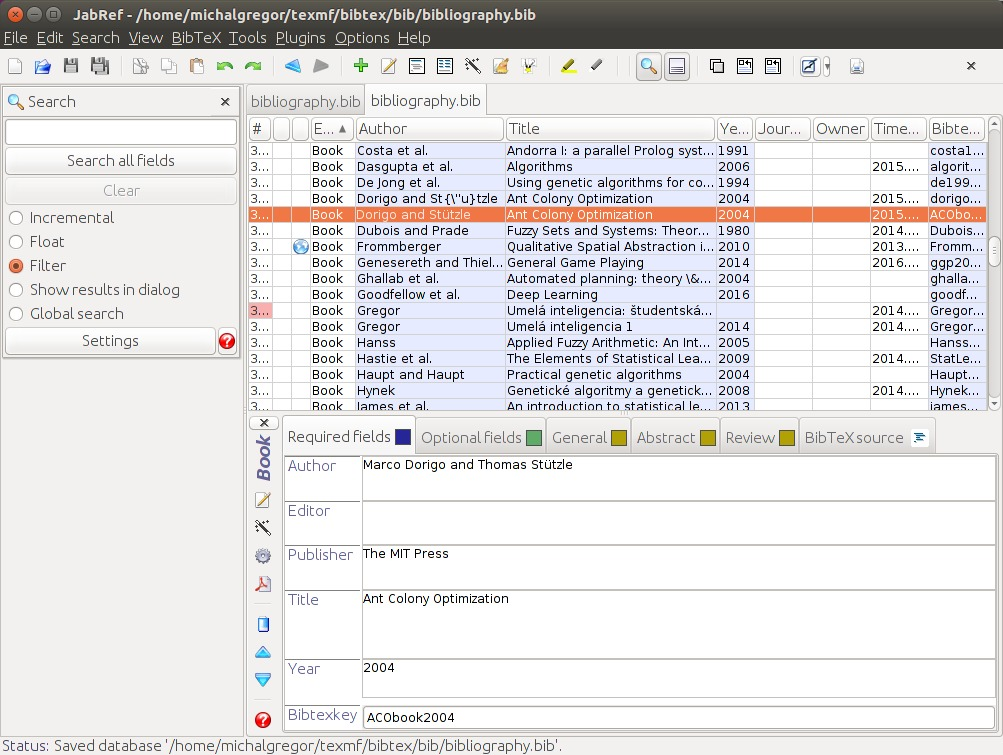
\includegraphics[width=\textwidth]{jabref}
\caption{Prvý obrázok.}
\label{fig:mini1}
\end{minipage}\quad
\begin{minipage}[b]{0.38\textwidth}
\centering

\includegraphics[width=\textwidth]{logo}
\caption{Druhý obrázok.}
\label{fig:mini2}
\end{minipage}
\end{figure}
\end{inlinecode}

Výsledkom je viacero obrázkov uložených vedľa seba, ako to ukazujú \figurename~\ref{fig:mini1} a \figurename~\ref{fig:mini2}.

\begin{figure}
\centering
\begin{minipage}[b]{0.58\textwidth}
\centering
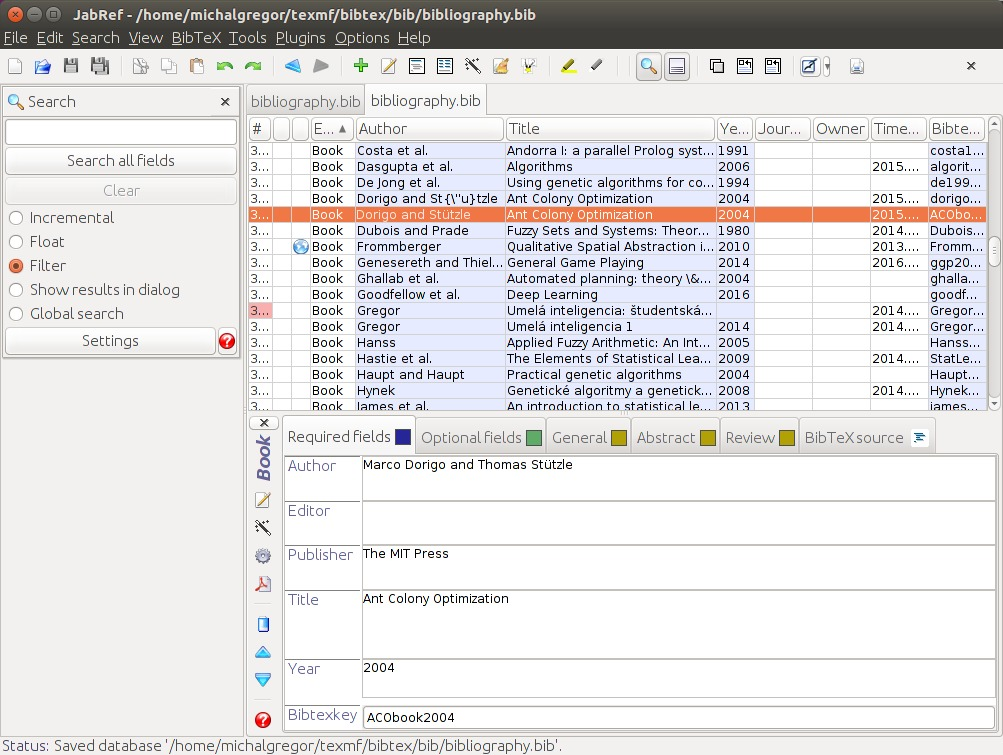
\includegraphics[width=\textwidth]{jabref}
\caption{Prvý obrázok.}
\label{fig:mini1}
\end{minipage}\quad
\begin{minipage}[b]{0.38\textwidth}
\centering

\includegraphics[width=\textwidth]{logo}
\caption{Druhý obrázok.}
\label{fig:mini2}
\end{minipage}
\end{figure}

Ako vidno, do toho istého \texttt{figure} prostredia sme vložili dve \texttt{minipage} prostredia -- jedno pre každý obrázok. Povinným argumentom \texttt{minipage} prostredia je jeho šírka -- časť strany sme nechali jednému a časť druhému obrázku a nejaké miesto sme vynechali aj pre medzeru medzi nimi. Nepovinným argumentom, ktorý sa uvádza v hranatých zátvorkách, je ako majú byť obrázky voči sebe vertikálne zarovnané. My sme zvolili možnosť \texttt{[b]}, t.j. majú byť zarovnané spodnou časťou.

\subsection{Podobrázky}

Obdobným spôsobom sa dajú vkladať podobrázky -- ibaže namiesto prostredia \texttt{minipage} sa použije prostredie \texttt{subfigure}. Príklad nasleduje tu:
\begin{inlinecode}{latex}
\begin{figure}
\centering
\begin{subfigure}[c]{0.5\textwidth}
	\centering
	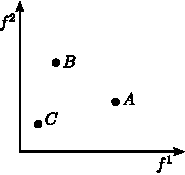
\includegraphics[width=6.5cm]{pareto_dominance}
	\caption{Pareto dominancia.}
	\label{fig:subfig1}
\end{subfigure}~
\begin{subfigure}[c]{0.5\textwidth}
	\centering
	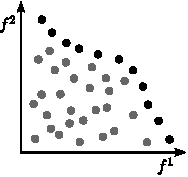
\includegraphics[width=6.5cm]{pareto_front}
	\caption{Pareto front.}
	\label{fig:subfig2}
\end{subfigure}
\caption{Ilustrácia: Pareto dominancia a Pareto front.}
\label{fig:fig_with_subfigs}
\end{figure}
\end{inlinecode}

Ako vidno na \figurename~\ref{fig:fig_with_subfigs}, obrázok má jeden spoločný popisok a takisto každý z podobrázkov má popisok, na ktorý sa dá odkazovať, napr. \figurename~\ref{fig:subfig1}.

\begin{figure}
\centering
\begin{subfigure}[c]{0.5\textwidth}
	\centering
	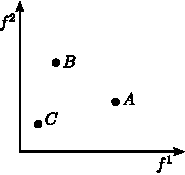
\includegraphics[width=6.5cm]{pareto_dominance}
	\caption{Pareto dominancia.}
	\label{fig:subfig1}
\end{subfigure}~
\begin{subfigure}[c]{0.5\textwidth}
	\centering
	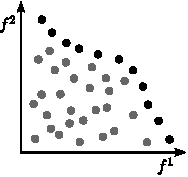
\includegraphics[width=6.5cm]{pareto_front}
	\caption{Pareto front.}
	\label{fig:subfig2}
\end{subfigure}
\caption{Ilustrácia: Pareto dominancia a Pareto front.}
\label{fig:fig_with_subfigs}
\end{figure}

\subsection{Vektorové a rastrové obrázky}

Vkladané obrázky by -- podľa možnosti -- mali mať vektorový formát. Platí to najmä v prípade schém, diagramov a pod. Rastrový formát obrázkov je prípustný v prípade, že ide o fotografie, screenshot-y alebo iné typy obrazového materiálu, ktoré majú prirodzene rastrovú formu. Rastrová forma je takisto vhodná v prípade nadštandardne zložitých obrázkov, ktorých vykresľovanie z vektorového formátu by pri zobrazovaní trvalo príliš dlho.

Najvhodnejšie formáty obrázkov pri použití v LaTeX-u sú zrejme \texttt{eps} a \texttt{pdf}. Existuje viacero dobrých nástrojov na tvorbu kvalitných vektorových obrázkov. Zdarma je k dispozícii napríklad nástroj Inkscape: \href{https://inkscape.org/en/}{inkscape.org}. Na editovanie rastrových obrázkov je zase možné použiť napríklad GIMP: \href{https://www.gimp.org/}{gimp.org}.

\subsection{Obrázky obtekané textom}

V odborných prácach sa spravidla nepoužívajú obrázky obtekané textom -- ich používanie neodporúčame ani v záverečnej práci. Navyše v LaTeX-u sa obtekanie dosahuje pomocou prostredia \texttt{wrapfigure}, ktoré je málo robustné a často spôsobuje nesprávne zalomenie textu a pod.

\subsection{Obrázky v landscape režime}

V prípade, že je potrebné vložiť obzvlášť veľký a široký obrázok (ktorý by nebol dostatočne čitateľný v zmenšenej podobe), je možné zobraziť ho na osobitnej strane v landscape režime. Používa sa na to prostredie \texttt{sidewaysfigure}, napr.:
\begin{inlinecode}{latex}
\begin{sidewaysfigure}[p]
\centering
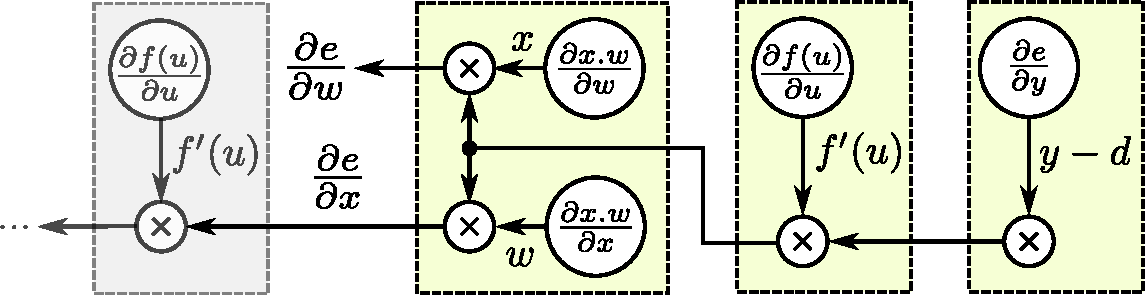
\includegraphics[width=23cm]{wide_figure}
\caption{Obzvlášť veľký a široký obrázok.}
\end{sidewaysfigure}
\end{inlinecode}

\begin{sidewaysfigure}[p]
\centering
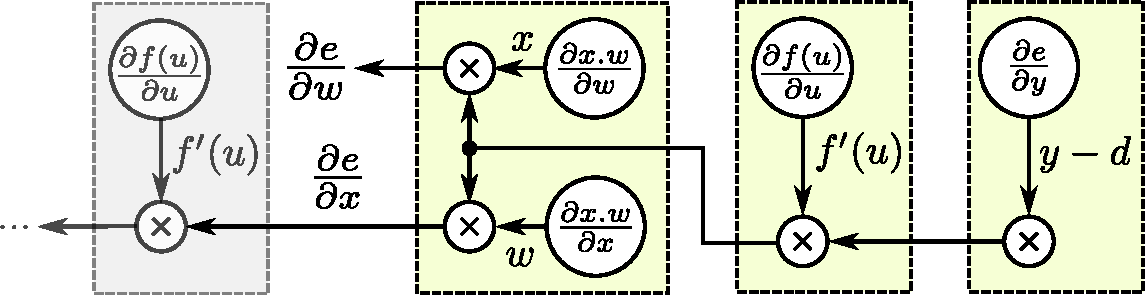
\includegraphics[width=23cm]{wide_figure}
\caption{Obzvlášť veľký a široký obrázok.}
\label{fig:wide_figure}
\end{sidewaysfigure}

Výsledok vidno na \figurename~\ref{fig:wide_figure}. Pre tabuľky existuje obdobné prostredie \texttt{sidewaystable}.

\section{Tabuľky}

Ďalší prvok, ktorý bude obsahovať väčšina záverečných prác, sú tabuľky. Vzhľadom na to, že tvorba tabuliek v LaTeX-u je pomerne komplikovaná, nebudeme sa na tomto mieste zaoberať všetkými detailami -- uvedieme len niekoľko základných ukážok. Iné príklady je možné nájsť povedzme v \cite{latexTables}.

Začnime jednoduchým príkladom: \tablename~\ref{tab:priklad}. Túto tabuľku je možné vygenerovať pomocou nasledujúceho kódu:
\begin{inlinecode}{latex}
\begin{table}
\centering
\caption{Príklad jednoduchej tabuľky.}
\label{tab:priklad}
\begin{tabular}{|l|c|r|}
\hline
\textbf{č. 1} & \textbf{č. 2} &  \textbf{č. 3} \\
\hline
1 & 2 & 3 \\
11 & 22 & 33 \\
111 & 222 & 333 \\
\hline
\end{tabular}
\end{table}
\end{inlinecode}
Odkaz na tabuľku sa píše v tvare:
\begin{inlinecode}{latex}
\tablename~\ref{tab:priklad}
\end{inlinecode}

Ako vidno, celá tabuľka je obalená do prostredia \texttt{table}. Toto prostredie je plávajúce -- čiže podobne ako v prípade obrázkov sa mu pozícia určuje automaticky. Samotné jadro tabuľky sa tvorí pomocou prostredia \texttt{tabular}. Jeho prvým argumentom je formátovanie stĺpcov. Pre každý stĺpec tabuľky tu vystupuje jedno písmenko, ktoré určuje zarovnanie (\texttt{l} -- doľava, \texttt{c} -- na stred, \texttt{r} -- doprava). Zvislé čiary medzi stĺpcami znamenajú zvislé orámovanie.

\begin{table}
\centering
\caption{Príklad jednoduchej tabuľky.}
\label{tab:priklad}
\begin{tabular}{|l|c|r|}
\hline
\textbf{č. 1} & \textbf{č. 2} &  \textbf{č. 3} \\
\hline
1 & 2 & 3 \\
11 & 22 & 33 \\
111 & 222 & 333 \\
\hline
\end{tabular}
\end{table}

Samotné riadky tabuľky sa vpisujú do vnútra prostredia \texttt{tabular}. Jednotlivé bunky sú od seba oddelené ampersandmi \& a každý riadok je ukončený značkou \textbackslash\textbackslash. Horizontálne orámovanie sa dá vložiť pomocou príkazu \texttt{{\textbackslash}hline}.

%TODO: Viac ku tabuľkám.

%\subsection{Horizontálne zlučovanie buniek}
%
%
%
%\subsection{Vertikálne zlučovanie buniek}
%
%
%
%\subsection{Lomené bunky}
%
%
%
%\subsection{Dlhé tabuľky}
%
%
%\todo[inline]{Dokončiť; pridať aj zložitejšie príklady s lomenými bunkami, krajšie formátovanými tabuľkami, multirow a multicol prípadmi a pod. longtable}


\section{Zoznam obrázkov a tabuliek}

Zoznam obrázkov a tabuliek sa v našej šablóne generuje automaticky. Obsahuje len obrázky/tabuľky, ktoré majú popisky. Vygeneruje sa len v tom prípade, že dokument naozaj nejaký obrázok/tabuľku obsahuje.

\section{Skratky a slovník pojmov}
\label{sec:skratky}

Práca má obsahovať zoznam skratiek a (nepovinne) slovník pojmov. Oba sa dajú generovať automaticky. Význam skratky sa najprv definuje v súbore \texttt{modules/abbterms.tex}. V texte sa skratka následne obalí do makra \texttt{ac}. Výsledkom je, že každá označená skratka obsahuje hypertextový odkaz na svoju definíciu v zozname skratiek a takisto, že do zoznamu skratiek pribudne číslo strany, na ktorej sa skratka použila.

Zmysel skratky je okrem toho potrebné vysvetliť v texte na tom mieste, kde sa prvýkrát používa -- nestačí len uviesť vysvetlenie v zozname skratiek. Napr. pri prvom použití povieme: umelá neurónová sieť (\angl{artificial neural network}; \ac{ANN}). Pri ďalšom použití stačí už len \ac{ANN}.

Obsah slovníka pojmov sa takisto vypĺňa v súbore \texttt{modules/abbterms.tex}, ale na pojmy sa nie je potrebné odkazovať z textu. V slovníku budú automaticky všetky zadefinované pojmy.

\section{Rovnice}

LaTeX má osobitne dobrú podporu pre sádzanie matematických výrazov, vkladanie rovníc s automatickým číslovaním a pod. Vkladanie rovníc je veľmi jednoduché a rýchle -- akonáhle sa užívateľ naučí základy syntaxe, ktorá je potrebná na ich zápis.

Matematické symboly a vzorce, ktoré majú byť súčasťou bežného textu sa označujú párom dolárov a zobrazujú sa nasledovne: $x^2 + \alpha$. Tento odsek by sa teda dal zapísať nasledujúcim spôsobom:
\begin{inlinecode}{latex}
Matematické symboly a vzorce, ktoré majú byť súčasťou bežného
textu sa označujú párom dolárov a zobrazujú sa nasledovne: $x^2 + \alpha$.
Tento odsek by sa teda dal zapísať nasledujúcim spôsobom:
\end{inlinecode}

Rovnice, ktoré sa majú zobrazovať osobitne, mimo riadku a majú byť číslované, sa dajú vložiť pomocou prostredia \texttt{equation}. Vyzerajú nasledovne:
\begin{equation}
x^2 + \alpha,
\label{eq:dolezita_rovnica}
\end{equation}
kde $x$ je premenná a $\alpha$ je konštanta.

Ak do rovnice vložíme návestie pomocou príkazu \texttt{label}, napr.:
\begin{inlinecode}{latex}
\begin{equation}
x^2 + \alpha,
\label{eq:dolezita_rovnica}
\end{equation}
\end{inlinecode}
môžeme sa na rovnicu odkázať z textu pomocou príkazu \texttt{{\textbackslash}eqref}, t.j.:
\begin{inlinecode}{latex}
Odkaz na rovnicu \eqref{eq:dolezita_rovnica} z textu.
\end{inlinecode}

Výsledný odkaz sa zobrazí nasledovne: Odkaz na rovnicu \eqref{eq:dolezita_rovnica} z textu.

\subsection{Odseky pokračujúce za rovnicou}

Všimnite si, že text nasledujúci za rovnicou nie je odsadený. Nejde totiž o nový odsek, ale o pokračovanie predošlého odseku -- dokonca o pokračovanie tej istej vety. Ak má LaTeX text interpretovať takto, nesmie sa za prostredím equation vynechať nový riadok, t.j. kód bude vyzerať takto:
\begin{inlinecode}{latex}
Rovnice, ktoré sa majú zobrazovať osobitne, mimo riadku a majú byť číslované, sa dajú vložiť pomocou prostredia \texttt{equation}. Vyzerajú nasledovne:
\begin{equation}
x^2 + \alpha,
\end{equation}
kde $x$ je premenná a $\alpha$ je konštanta.
\end{inlinecode}

Keby sa nový riadok vynechal, bude LaTeX text za rovnicou interpretovať už ako nový odsek a výsledok bude nasledovný:
\begin{equation}
x^2 + \alpha,
\end{equation}
% tento prázdny riadok je tu úmyselne
	
kde $x$ je premenná a $\alpha$ je konštanta.

\subsection{Viacero rovníc pod sebou}

LaTeX poskytuje aj dobré nástroje na zobrazovanie viacerých rovníc pod sebou. Je ich možné zobraziť buď centrované -- pomocou prostredia \texttt{gather} -- alebo zarovnané -- pomocou prostredia \texttt{align}.

Centrované rovnice môžu vyzerať nasledovne:
\begin{gather}
x = 2a - 3b \\
y = x^2.
\end{gather}

Kód potrebný na ich zobrazenie vyzerá takto:
\begin{inlinecode}{latex}
\begin{gather}
x = 2a - 3b \\
y = x^2.
\end{gather}
\end{inlinecode}

Zarovnané rovnice môžu zase vyzerať napríklad takto:
\begin{align}
x &= 2a - 3b \\
y &= x^2.
\end{align}

Kód potrebný na ich zobrazenie vyzerá nasledovne:
\begin{inlinecode}{latex}
\begin{align}
x &= 2a - 3b \\
y &= x^2.
\end{align}
\end{inlinecode}

Alternatívne sa dajú použiť prostredia \texttt{gathered} a \texttt{aligned} -- ide o alternatívy, ktoré sa používajú zvnútra prostredia \texttt{equation}. Rovnica sa potom správa ako jeden celok a má len jedno spoločné číslovanie. Číslovanie sa dá potlačiť pre jednotlivé riadky rovnice aj použitím makra \texttt{{\textbackslash}notag}.

\section{Úvodzovky}

Vzhľadom na to, že v každom jazyku sa úvodzovky zapisujú trochu inak, obsahuje LaTeX makro \texttt{enquote} (z balíčka \texttt{csquotes}), ktoré správnu formu úvodzoviek pre daný jazyk generuje. Text, ktorý má byť v úvodzovkách sa teda obalí do makra \texttt{enquote} takto:
\begin{inlinecode}{latex}
\enquote{Text v úvodzovkách}
\end{inlinecode}

Výsledok môže vyzerať napríklad nasledovne: \enquote{Text v úvodzovkách}. Úvodzovky majú viacero úrovní, takže makro \texttt{enquote} môže byť aj vnorené, napr.: \enquote{Text vo vonkajších úvodzovkách, \enquote{text vo vnútorných úvodzovkách}.}

Mnohé LaTeX-ové editory majú pre \texttt{enquote} vstavanú podporu, takže priamo pri písaní vkladajú namiesto úvodzoviek rovno toto makro.

\section{Zoznamy}

Ďalej treba vedieť, ako sa v LaTeX-u zapisujú zoznamy. Existuje ich niekoľko typov -- na prvom mieste ide o číslované a nečíslované zoznamy -- ale v tejto podkapitole sa pozrieme aj na niektoré ďalšie.

\subsection{Číslované zoznamy}

Číslované zoznamy sa vytvárajú pomocou prostredia \texttt{enumerate}, napr.:
\begin{inlinecode}{latex}
\begin{enumerate}
\item položka,
\item položka,
\item položka.
\end{enumerate}
\end{inlinecode}

Zoznam sa zobrazí nasledovne:
\begin{enumerate}
\item položka,
\item položka,
\item položka.
\end{enumerate}

\subsection{Nečíslované zoznamy}

Úplne obdobne sa vytvárajú nečíslované zoznamy -- ibaže sa použije prostredie \texttt{itemize}. Výsledok môže vyzerať nasledovne:
\begin{itemize}
\item položka,
\item položka,
\item položka.
\end{itemize}

\subsection{Viacstĺpcové zoznamy}

V prípade, že zoznam obsahuje viacero položiek, ktoré v horizontálnom smere nezaberajú veľa miesta, môže byť lepšie usporiadať ich do viacerých stĺpcov. V tom prípade sa dá celý zoznam obaliť do prostredia \texttt{multicols} nasledujúcim spôsobom:
\begin{inlinecode}{latex}
\begin{multicols}{2}
\begin{itemize}
\item položka,
\item položka,
\item položka,
\item položka,
\item položka,
\item položka.
\end{itemize}
\end{multicols}
\end{inlinecode}

Výsledný zoznam bude mať teraz dva stĺpce:
\begin{multicols}{2}
\begin{itemize}
\item položka,
\item položka,
\item položka,
\item položka,
\item položka,
\item položka.
\end{itemize}
\end{multicols}

\subsection{Inline zoznamy}

V rámci šablóny definujeme aj zoznam \texttt{inlinelist}, ktorý sa zobrazuje inline -- t.j. vo vnútri riadku, napr.:
\begin{inlinelist}
\item položka,
\item položka,
\item položka.
\end{inlinelist}

\section{Poznámky pod čiarou}

Poznámky pod čiarou možno vložiť pomocou príkazu \texttt{footnote}, napr.\footnote{Poznámka pod čiarou.}:
\begin{inlinecode}{latex}
\footnote{Poznámka pod čiarou.}
\end{inlinecode}

Eventuálne je možné pomocou príkazu \texttt{footnotemark} označiť miesto, ku ktorému poznámka patrí a nižšie pomocou príkazu \texttt{footnotetext} definovať jej obsah -- to je užitočné najmä v prípade dlhších poznámok.

\section{Algoritmy}

Algoritmy je možné do práce vkladať buď v podobe pseudokódu, v podobe vývojového diagramu alebo v podobe konkrétneho zdrojového kódu. Vývojové diagramy sa prirodzene vkladajú ako klasické obrázky. Zvyšnými dvomi typmi zobrazenia sa budeme zaoberať v tejto podkapitole.

\subsection{Pseudokód}

Začneme pseudokódom. Pre LaTeX existuje viacero balíčkov na sádzanie pseudokódov. Dobré výsledky možno dosiahnuť napr. pomocou balíčka \texttt{algorithm2e}, ktorý je už include-ovaný do šablóny. Pseudokód možno pomocou neho zapísať napríklad nasledovne:
\begin{inlinecode}{text}
\begin{algorithm}
Zvoliť počiatočné hodnoty pre parametre: $a_0$, $c_0$\;
\For{$k = 1 \text{ až } pocet\_krokov$}{

$\Delta_a \leftarrow 0$; $\Delta_c \leftarrow 0$\;

\ForEach{$(x, d) \in P$}{
	$\Delta_a \leftarrow \Delta_a - \gamma
	\frac{\partial E(x, d, a_{k-1}, c_{k-1})}{\partial a}$\; 
	$\Delta_c \leftarrow \Delta_c - \gamma
	\frac{\partial E(x, d, a_{k-1}, c_{k-1})}{\partial c}$\;
}

$a_{k} = a_{k-1} + \Delta_a$\;
$c_{k} = c_{k-1} + \Delta_c$\;
}
\caption{Príklad pseudokódu.}
\label{alg:graddesc_iterative}
\end{algorithm}
\end{inlinecode}
Výsledný pseudokód ukazuje \algorithmname~\ref{alg:pseducode}. Na pseudokódy sa odkazujeme pomocou kódu v tvare \texttt{{\textbackslash}algorithmname\textasciitilde{\textbackslash}ref\{alg:pseducode\}}.

\begin{algorithm}
Zvoliť počiatočné hodnoty pre parametre: $a_0$, $c_0$\;
\For{$k = 1 \text{ až } pocet\_krokov$}{

$\Delta_a \leftarrow 0$; $\Delta_c \leftarrow 0$\;

\ForEach{$(x, d) \in P$}{
	$\Delta_a \leftarrow \Delta_a - \gamma \frac{\partial E(x, d, a_{k-1}, c_{k-1})}{\partial a}$\; 
	$\Delta_c \leftarrow \Delta_c - \gamma \frac{\partial E(x, d, a_{k-1}, c_{k-1})}{\partial c}$\;
}

$a_{k} = a_{k-1} + \Delta_a$\;
$c_{k} = c_{k-1} + \Delta_c$\;
}
\caption{Príklad pseudokódu.}
\label{alg:pseducode}
\end{algorithm}

\subsection{Zdrojový kód}

Ak chceme vložiť zdrojový kód priamo, dá sa použiť prostredie \texttt{code} alebo \texttt{inlinecode} vstavané do šablóny. Ak vkladáme kratší zdrojový kód, ktorý nie je uložený v osobitnom súbore, ale ho budeme písať priamo do dokumentu, použijeme prostredie \texttt{inlinecode}, napr.:
\begin{Verbatim}
\begin{inlinecode}[label={lst:inline_code},
caption={Príklad krátkeho zdrojového kódu.}]{python}
def power(x):
	return x ** 2
\end{inlinecode}
\end{Verbatim}
Ako vidno, aby sa správne zvýraznila syntax, je potrebné zadať, v akom jazyku je kód napísaný. Ak sa syntax zvýrazňovať nemá, namiesto označenia jazyka sa napíše \texttt{text}. Argumenty v hranatých zátvorkách sú nepovinné. Ak zdrojový kód nemá mať titulok, stačí jednoducho vynechať nepovinný parameter \texttt{caption}.

Zdrojový kód sa zobrazí ako to vidno na \listingname~\ref{lst:inline_code}. Na zdrojové kódy sa odkazujeme pomocou zápisu v tvare \texttt{{\textbackslash}listingname\textasciitilde{\textbackslash}inline\_code}.

\begin{inlinecode}[label={lst:inline_code},
caption={Príklad krátkeho zdrojového kódu.}]{python}
def power(x):
	return x ** 2
\end{inlinecode}
Naopak pre prípad dlhších zdrojových kódov, ktoré sú uložené v osobitných súboroch, možno použiť prostredie \texttt{code}, napr.:
\begin{Verbatim}
\begin{code}
\caption{Ukážka dlhšieho zdrojového kódu.}
\inputcode[firstline=5,lastline=39]{python}
	{listings/delta_rule.py}
\label{lst:delta_rule}
\end{code}
\end{Verbatim}

Parametre uvedené v hranatých zátvorkách sú znovu nepovinné -- \texttt{firstline} a \texttt{lastline} určujú, aký rozsah riadkov sa má zobraziť. Ukážka výsledku je na \listingname~\ref{lst:delta_rule}.
\begin{code}
\caption{Ukážka dlhšieho zdrojového kódu.}
\inputcode[firstline=5,lastline=38]{python}
	{listings/delta_rule.py}
\label{lst:delta_rule}
\end{code}
Ak sa zo zdrojového kódu zobrazujú len niektoré riadky, treba pri prípadnom neskoršom editovaní kódu samozrejme dbať na to, aby sa riadky nepoposúvali.

\section{TODO poznámky}

Pri písaní záverečnej práce môže byť užitočné vložiť na niektoré rozpracované miesta TODO poznámky. Dá sa to realizovať pomocou príkazu \texttt{todo}, napr.:
\begin{inlinecode}{latex}
\todo[inline]{Príklad TODO poznámky.}
\end{inlinecode}

\todo[inline]{Príklad TODO poznámky.}
